%
% ---------- chapter 5 ----------
%

\section{Experimental Results}
%
To assess the evolutionary algorithm proposed in this paper, two separated
evaluation experiments are made for the efficiency of parallel evolutionary
algorithm and the validity of evolutionary algorithm in project management
problem. The purpose of the experiment is to answer the following two research
questions:


\textbf{RQ1}: Does the evolutionary algorithm effectively optimize project
management problem, and get an optimized answer?

\textbf{RQ2}: Is the parallel evolutionary algorithm able to improve the
efficiency in the project management problem?


\subsection{Industrial Project Data}
%
The experimental data evaluated in this paper are real industrial project
management plans.


There are three software project plannings, which are named as \emph{A-Input},
\emph{B-DBUpgrade} and \emph{C-SmartPrice}, where \emph{A-Input} is a simulated
medium-scale project planning. \emph{B-DBUpgrade} is the project plan of the
Oracle database upgrade. The goal of \emph{B-DBUpgrade} is to upgrade the Oracle
database from the \emph{9g} version to the \emph{10g} version, which is Oracle's
non-public version of the project planning. \emph{C-SmartPrice} is a
medium-sized project planning about supply chain upgrade, and like B, it is a
non-public of the internal project planning \cite{ren}. The configuration of the
projects is shown in Table \ref{tab:statis}.

\begin{figure}[!ht]
  \centering
  \subfigure[sub a]{
    \centering
    \label{fig:dag:a} 
    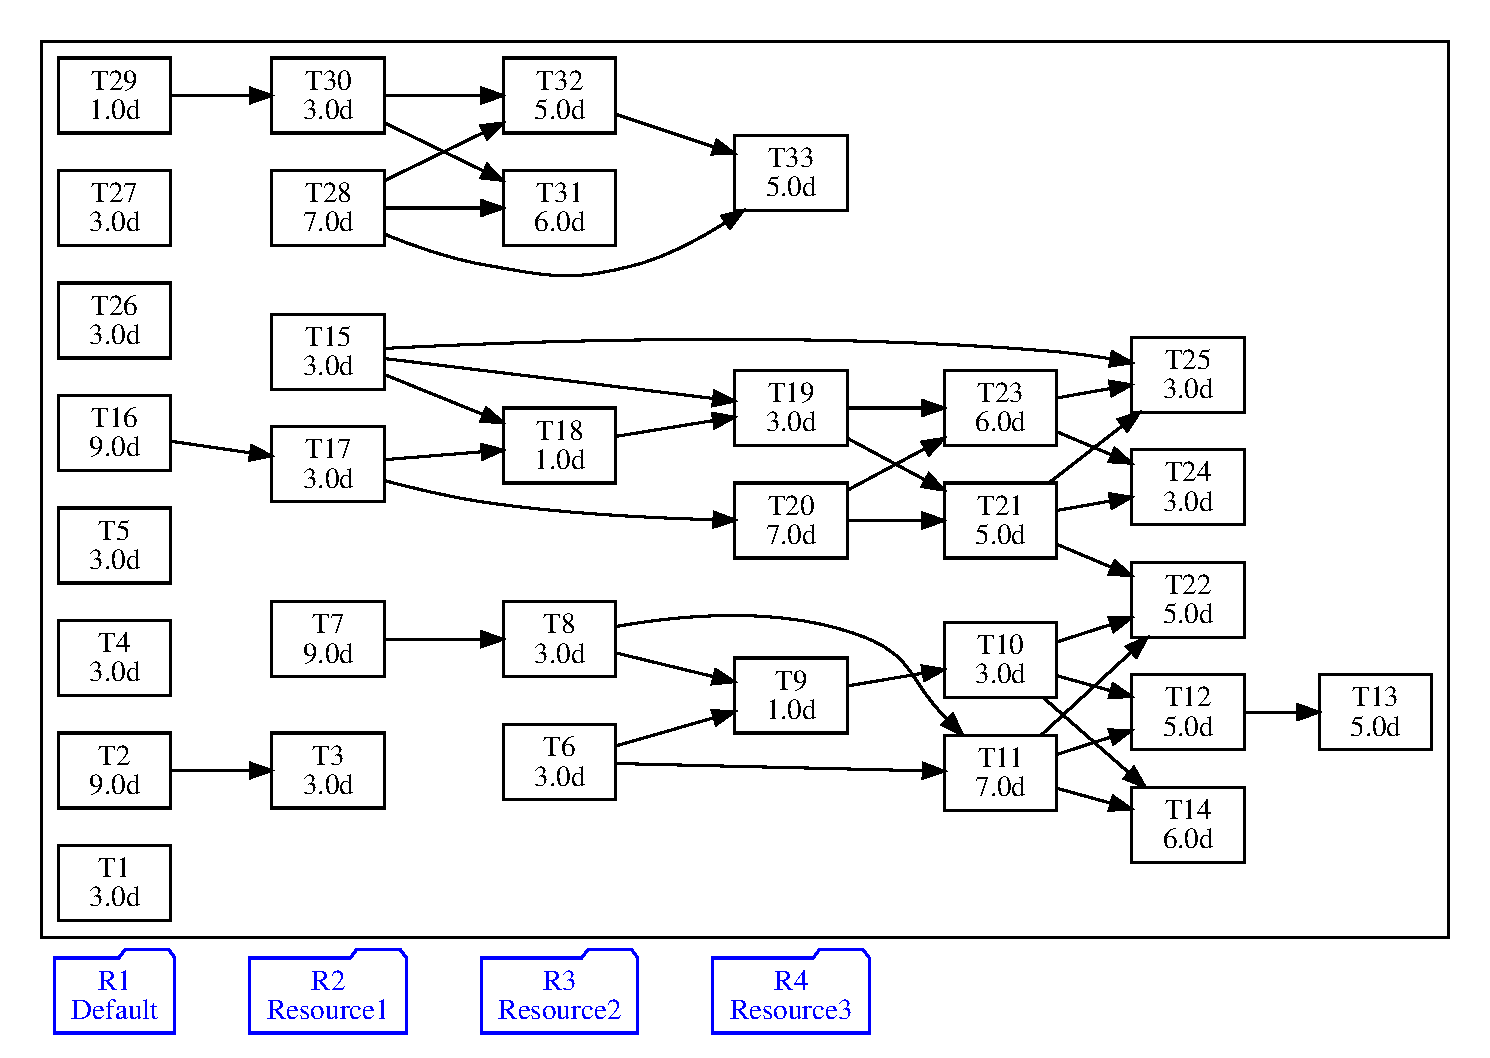
\includegraphics[width=\textwidth]{figures/a.eps}
  }
  \subfigure[sub b]{
    \centering
    \label{fig:dag:b}
    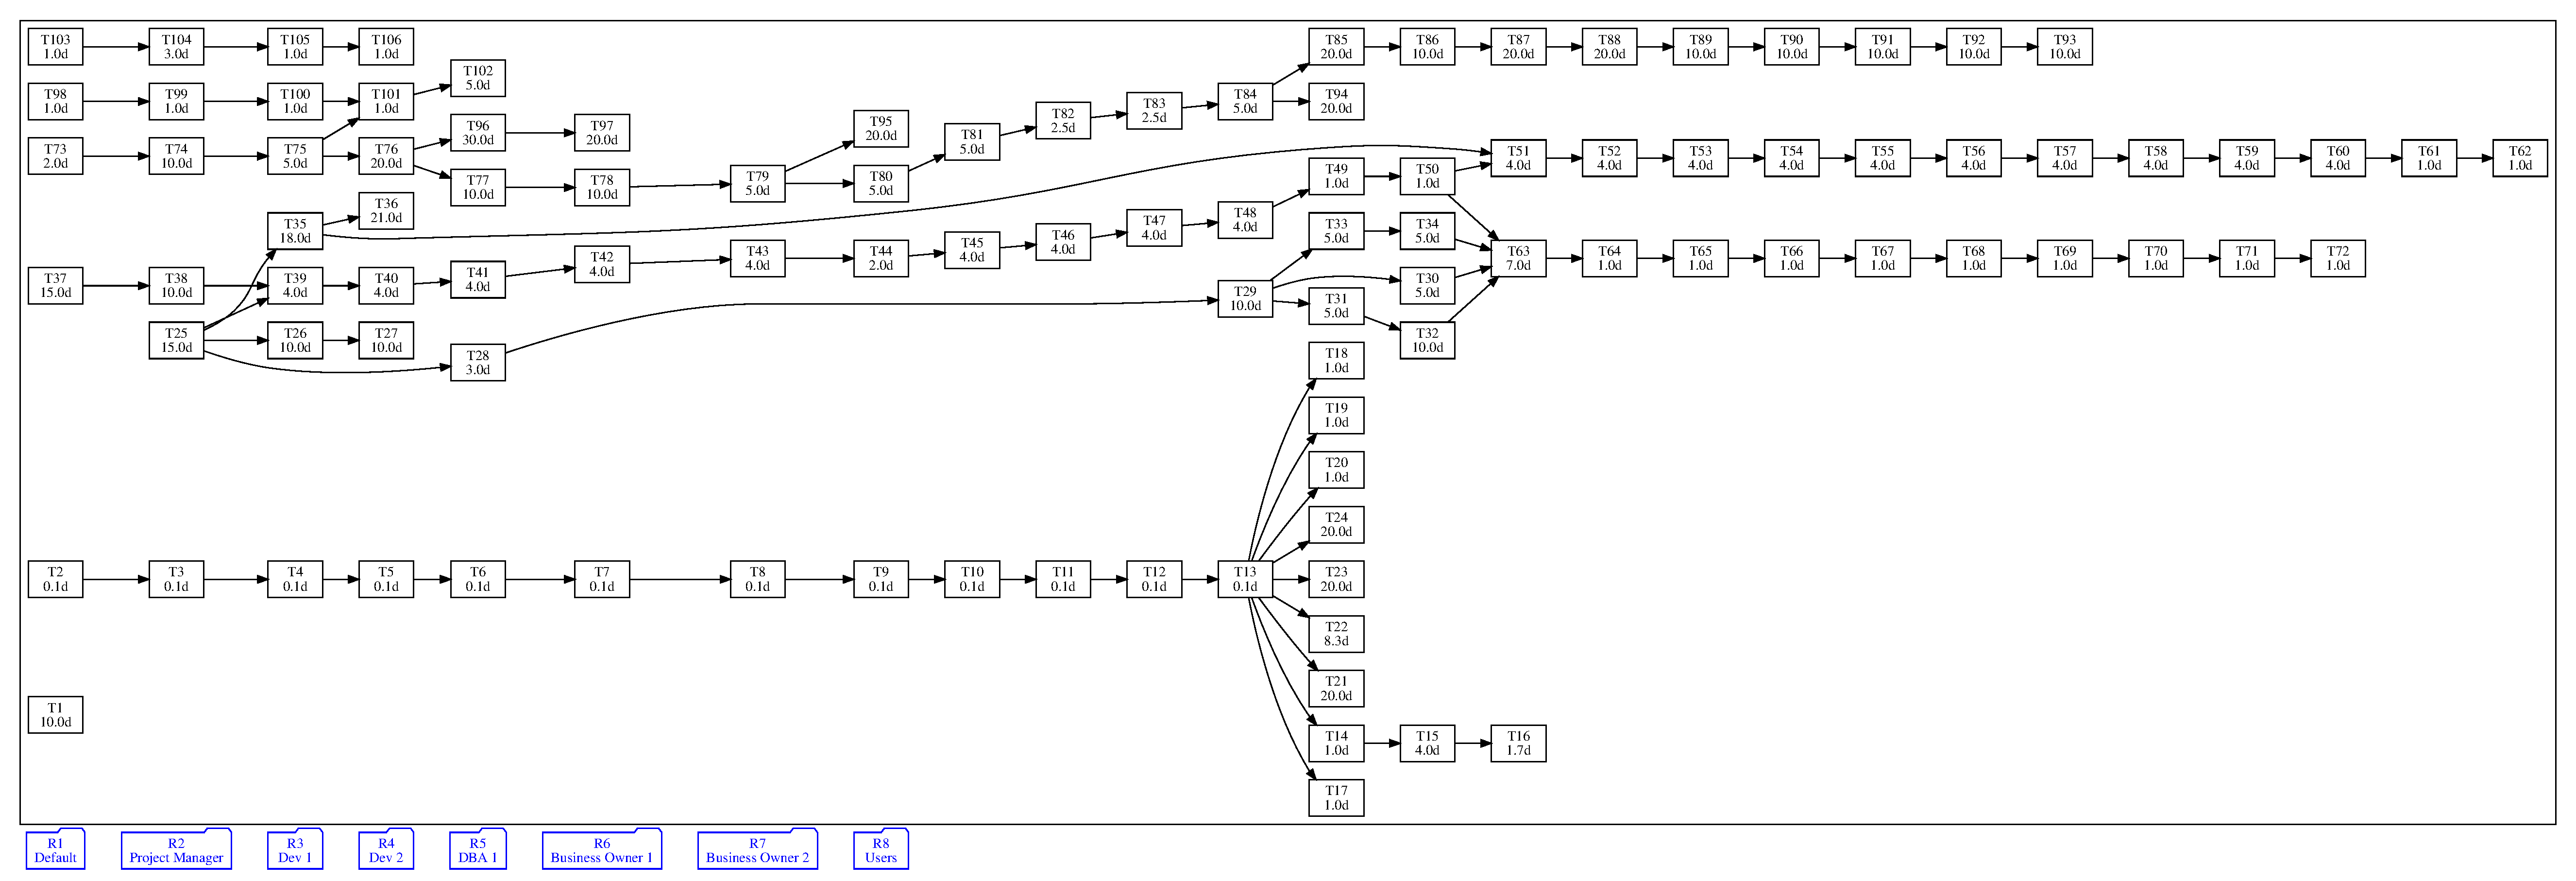
\includegraphics[width=\textwidth]{figures/b.eps}
  }
  \subfigure[sub c]{
    \centering
    \label{fig:dag:c}
    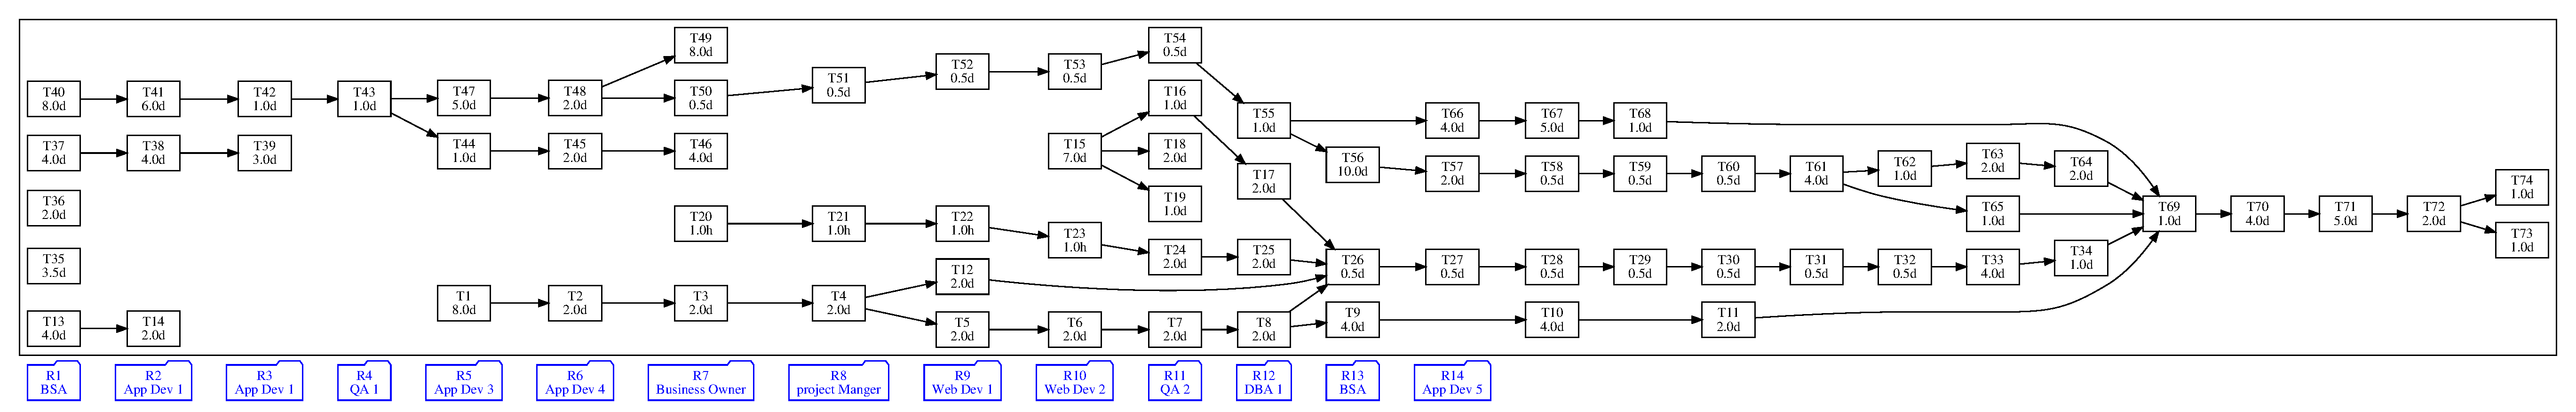
\includegraphics[width=\textwidth]{figures/c.eps}
  }
  \caption{caption a}
  \label{fig:dag}
\end{figure}


% 
\begin{table}[!h]
  \centering
  \caption{Three Project's Parameters}
  \label{tab:statis}
  \begin{tabular}{lccc}
    \hline
      & $\#$ work packages & $\#$ resources & $\#$ dependencies \\
    \hline
    \emph{A-Input}      & 33  & 4  & 33  \\
    \emph{B-DBUpgrade}  & 106 & 8  & 105 \\
    \emph{C-SmartPrice} & 74  & 14 & 73  \\
    \hline
  \end{tabular}
\end{table}


\subsection{Effectiveness Experiment for Algorithm}
%
In order to answer \textbf{RQ1}, this section designs a effectiveness experiment
for evolutionary algorithm. The basic configuration used in the experiment is
that \emph{100} individuals runs in \emph{50} generations. For each generation
in the evolutionary algorithm, we counts the each individuals' fitness value in
the whole population, and then plot the statistical data into a boxplot diagram.


Each generation of the boxplot shows the five statistical data of all
individuals' fitness value in the whole population: the minimum, the lower
quartile, the median, the upper quartile and the maximum. Boxplot about the
above-mentioned three industrial projects is shown in figures \ref{fig:pj}. From
the trend of three projects, it can be seen that the population is diversified
when the population is initialized. As the number of generation increase, all
the fitness value begins to decrease, and finally converges to a optimized
result.

\begin{figure}[ht]
  \centering
  \subfigure[Trend of \emph{A-Input}, solution converges in \emph{19th} generation]{
    \label{fig:pj:a} 
    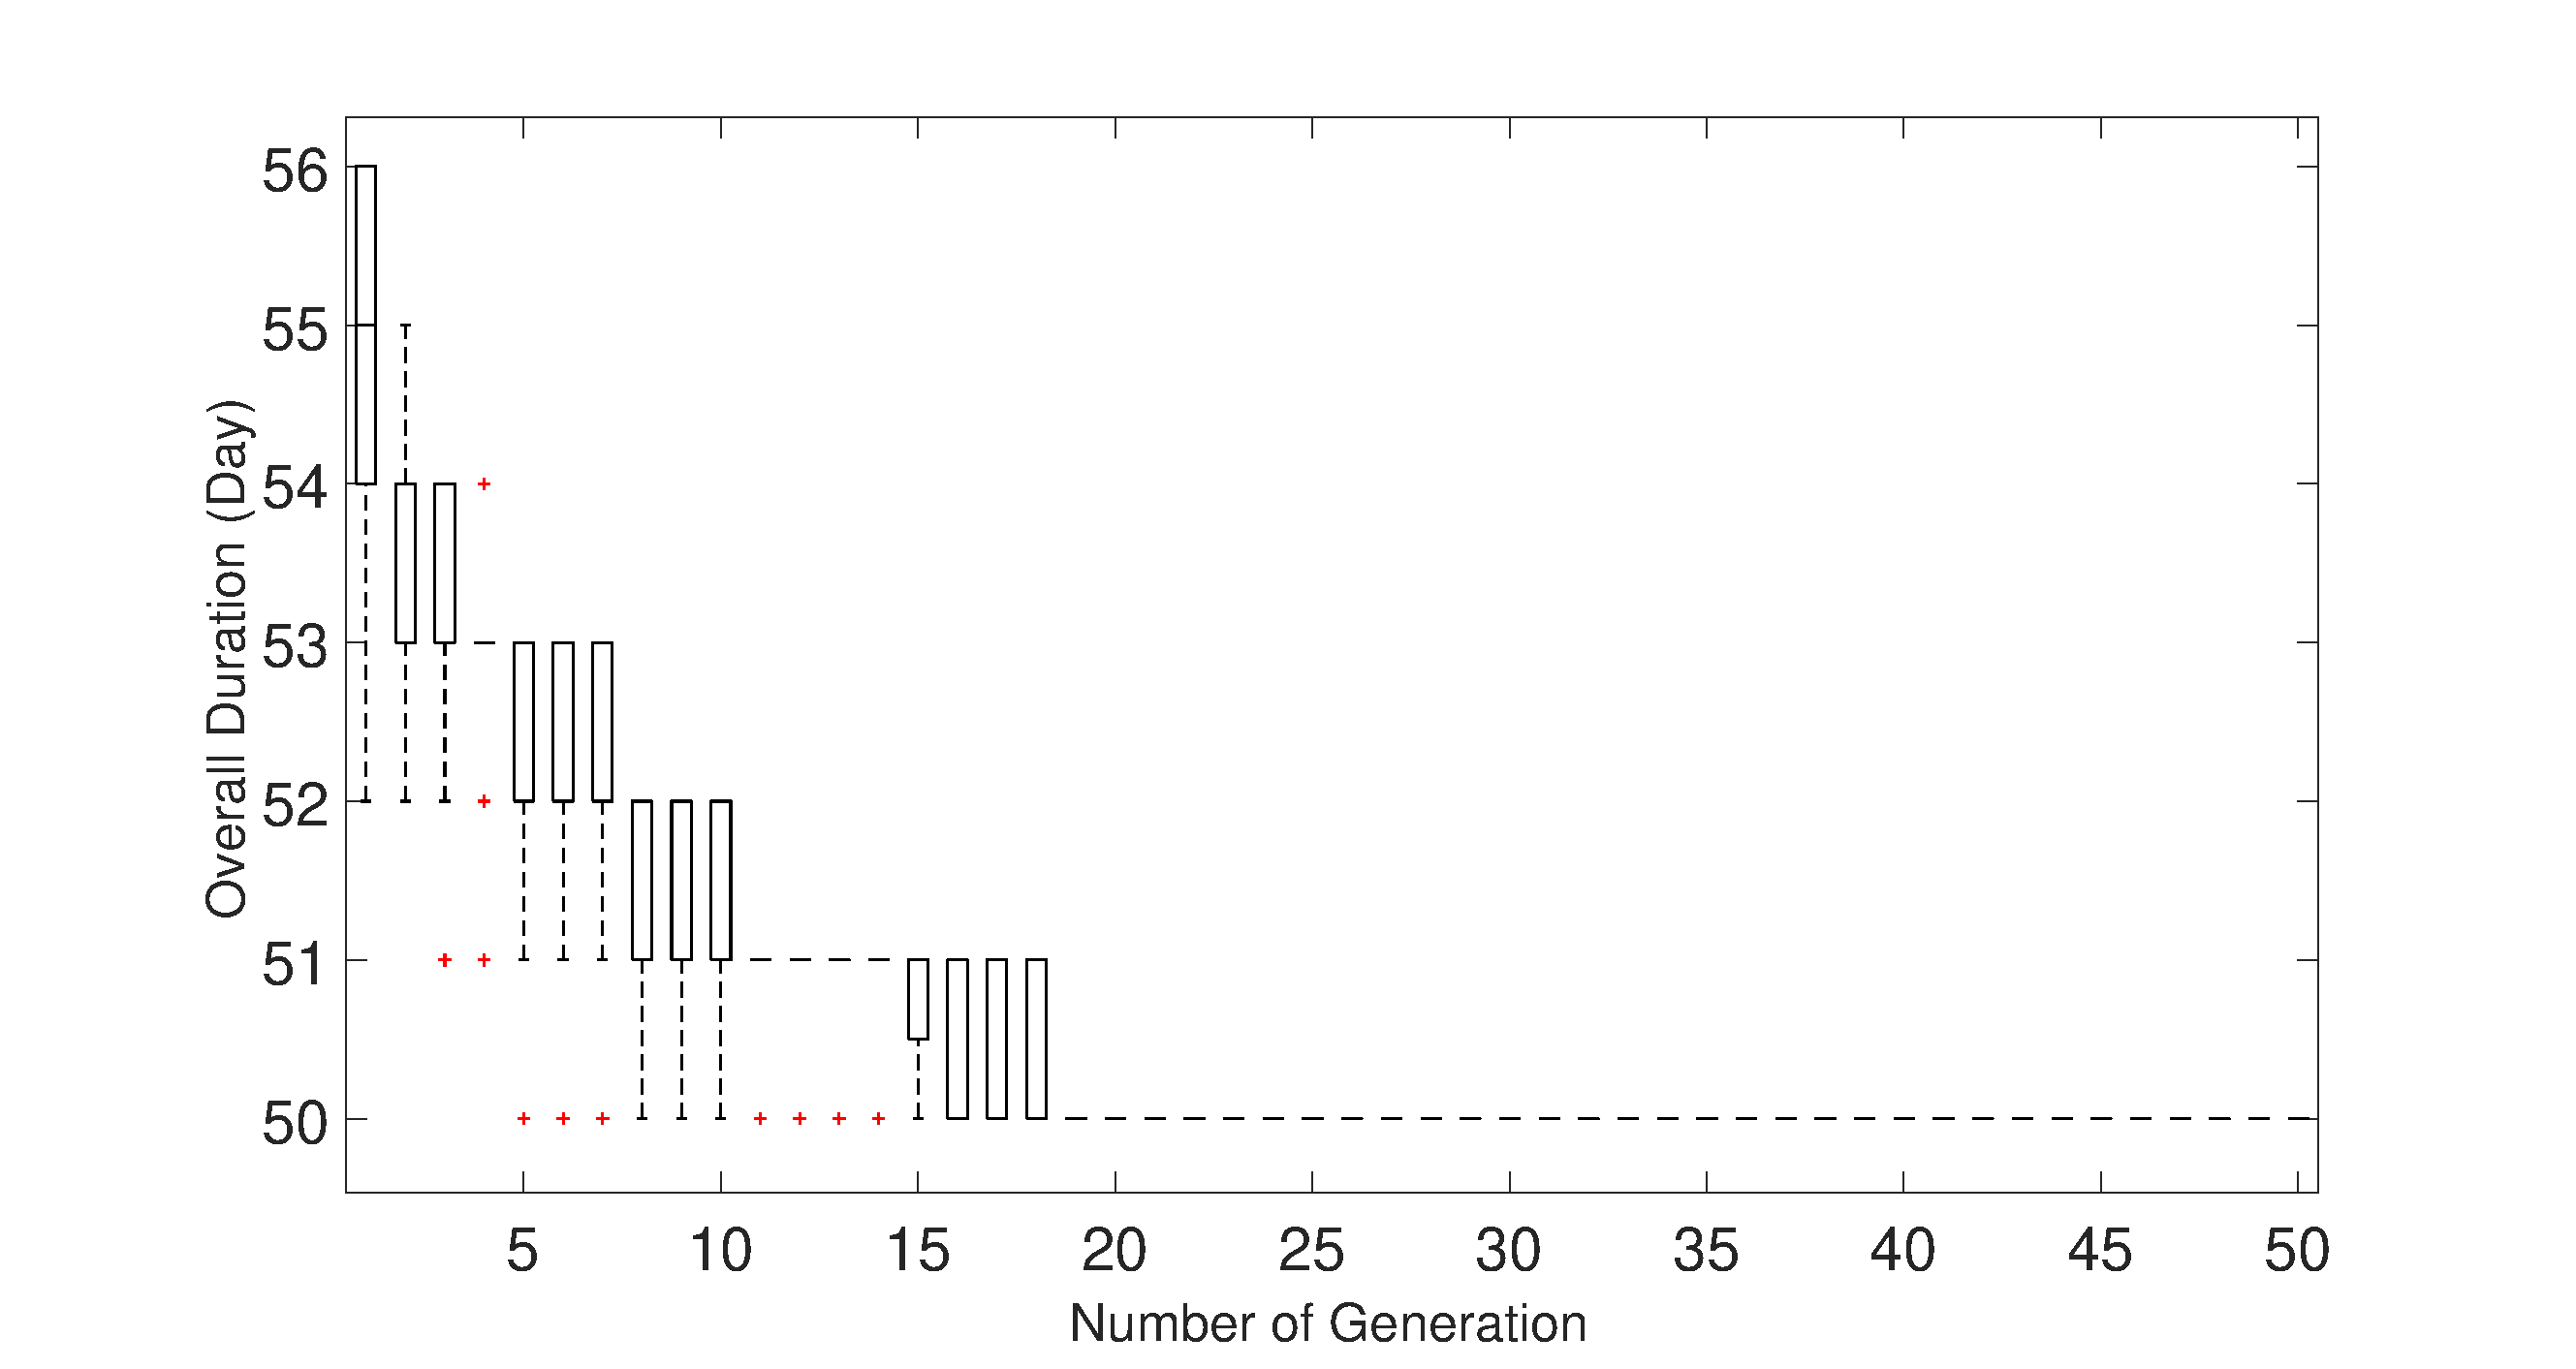
\includegraphics[width=0.8\textwidth]{figures/fig_pa1.eps}
  }
  \subfigure[Trend of \emph{B-DBUpgrade}, solution converges in \emph{22rd} generation]{
    \label{fig:pj:b} 
    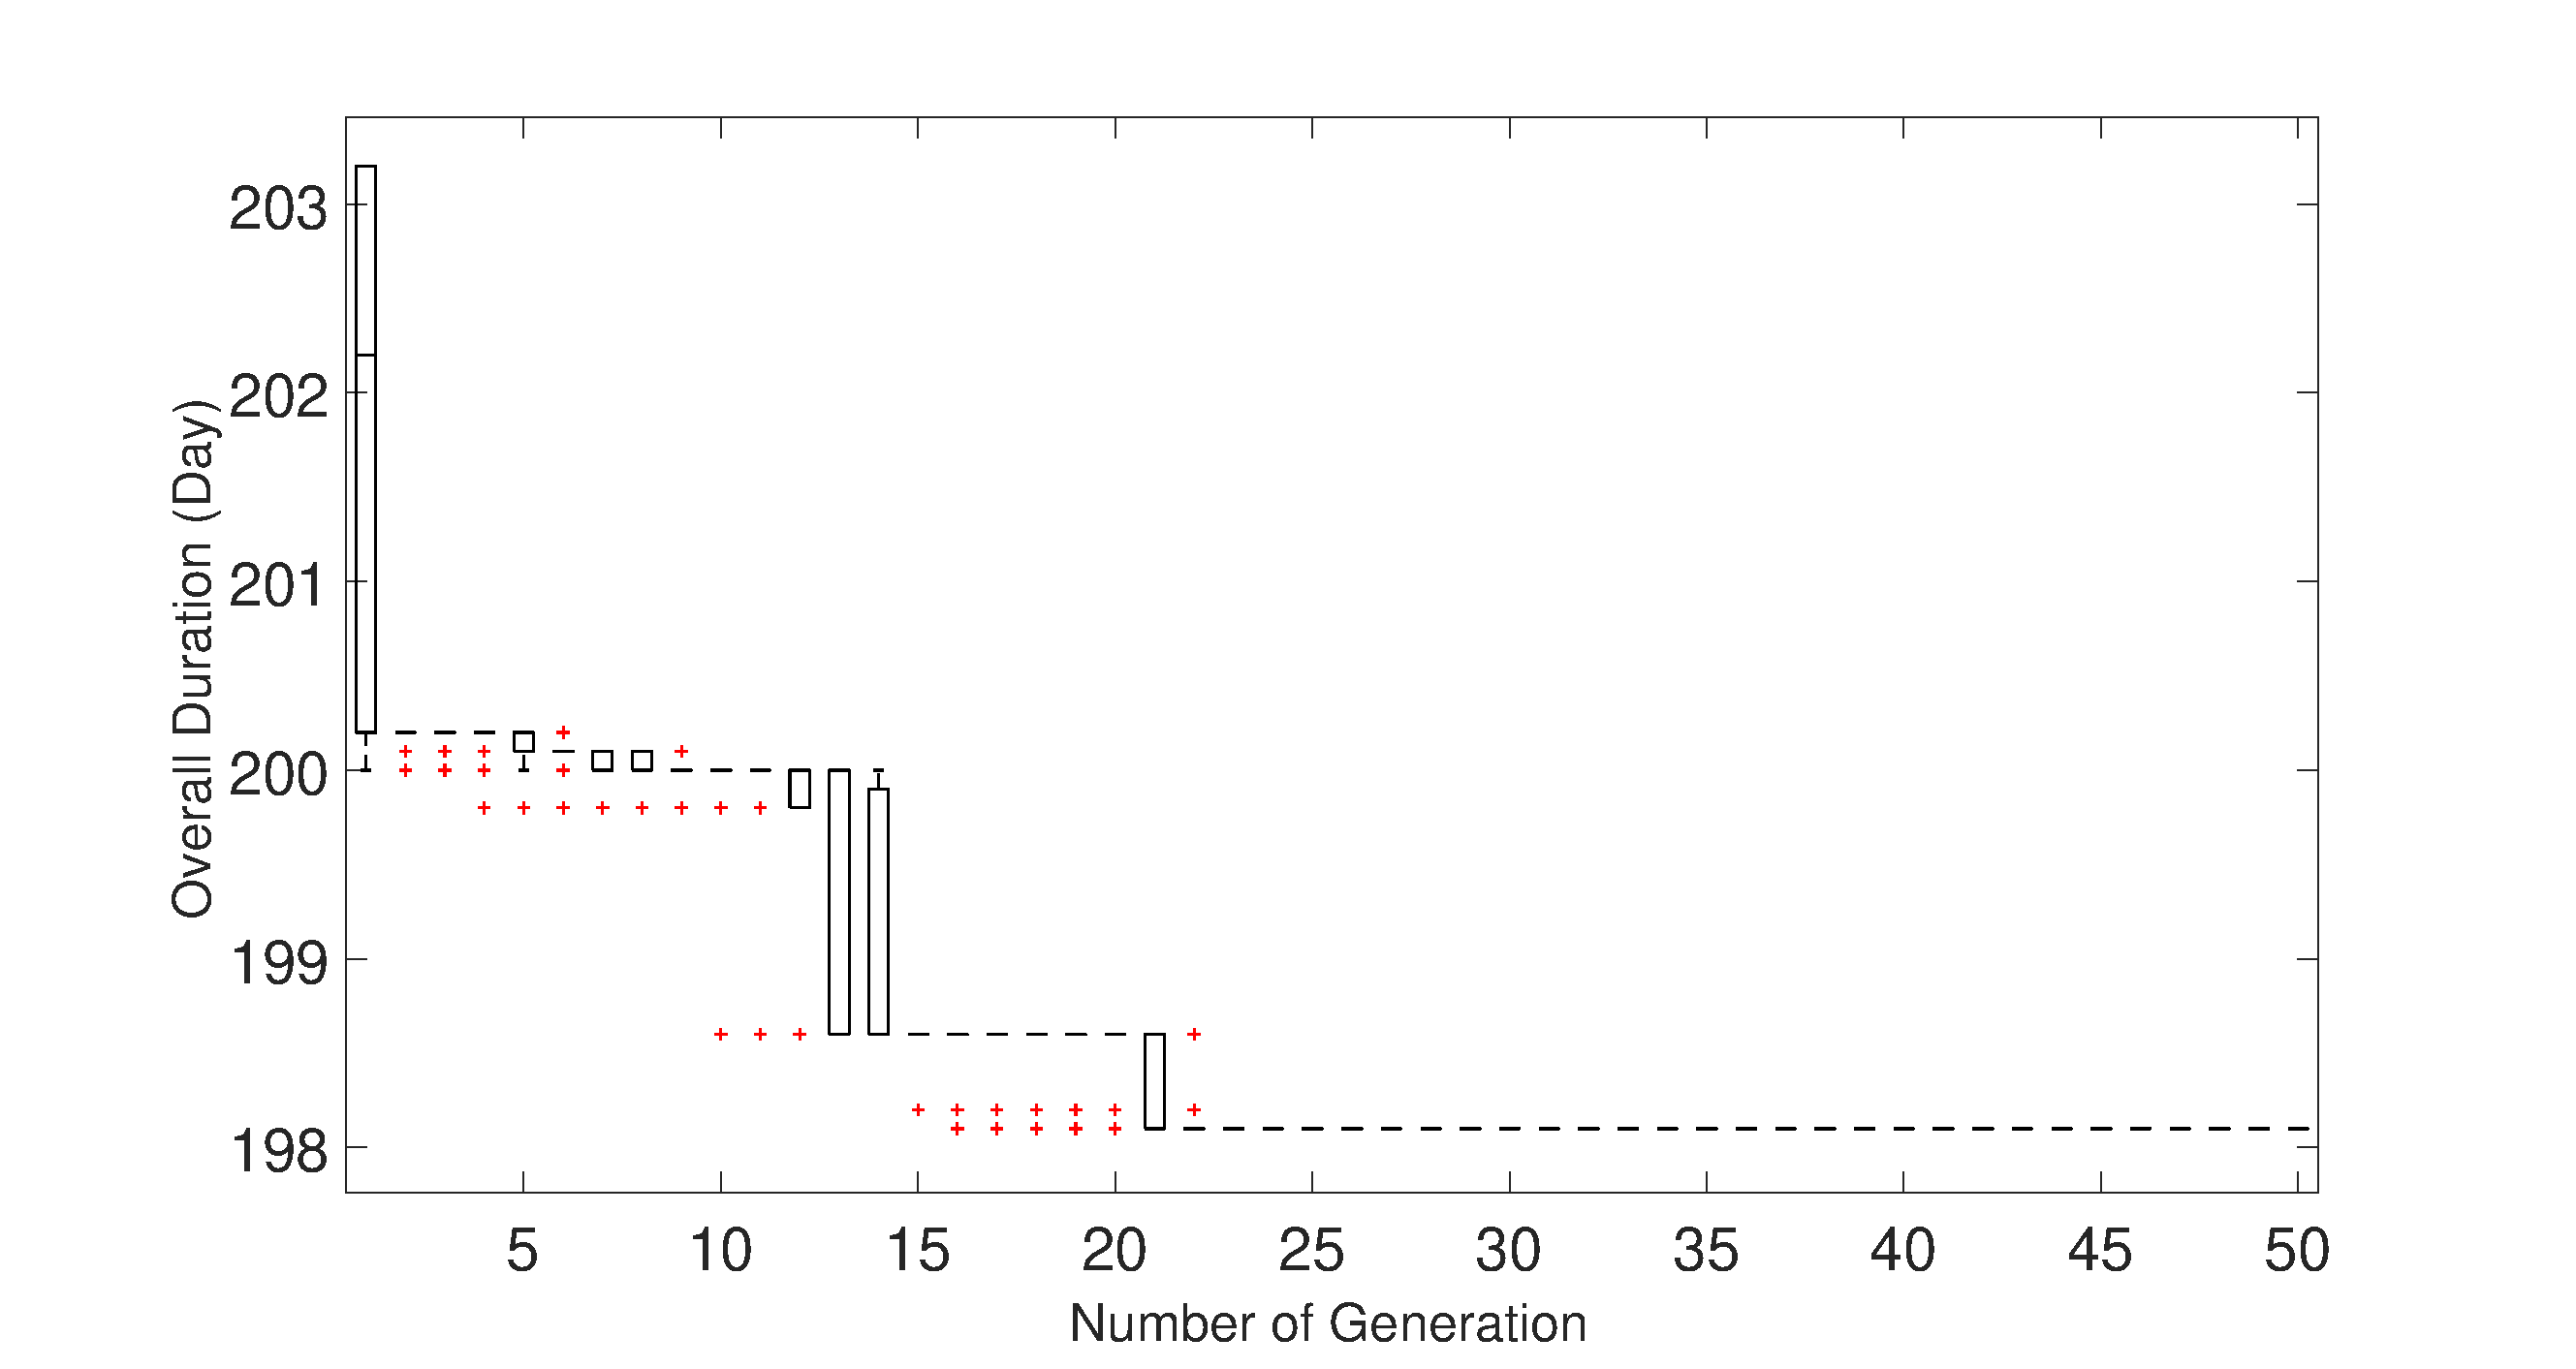
\includegraphics[width=0.8\textwidth]{figures/fig_pa2.eps}
  }
  \subfigure[Trend of \emph{A-Input}, solution converges in \emph{15th} generation]{
    \label{fig:pj:c} 
    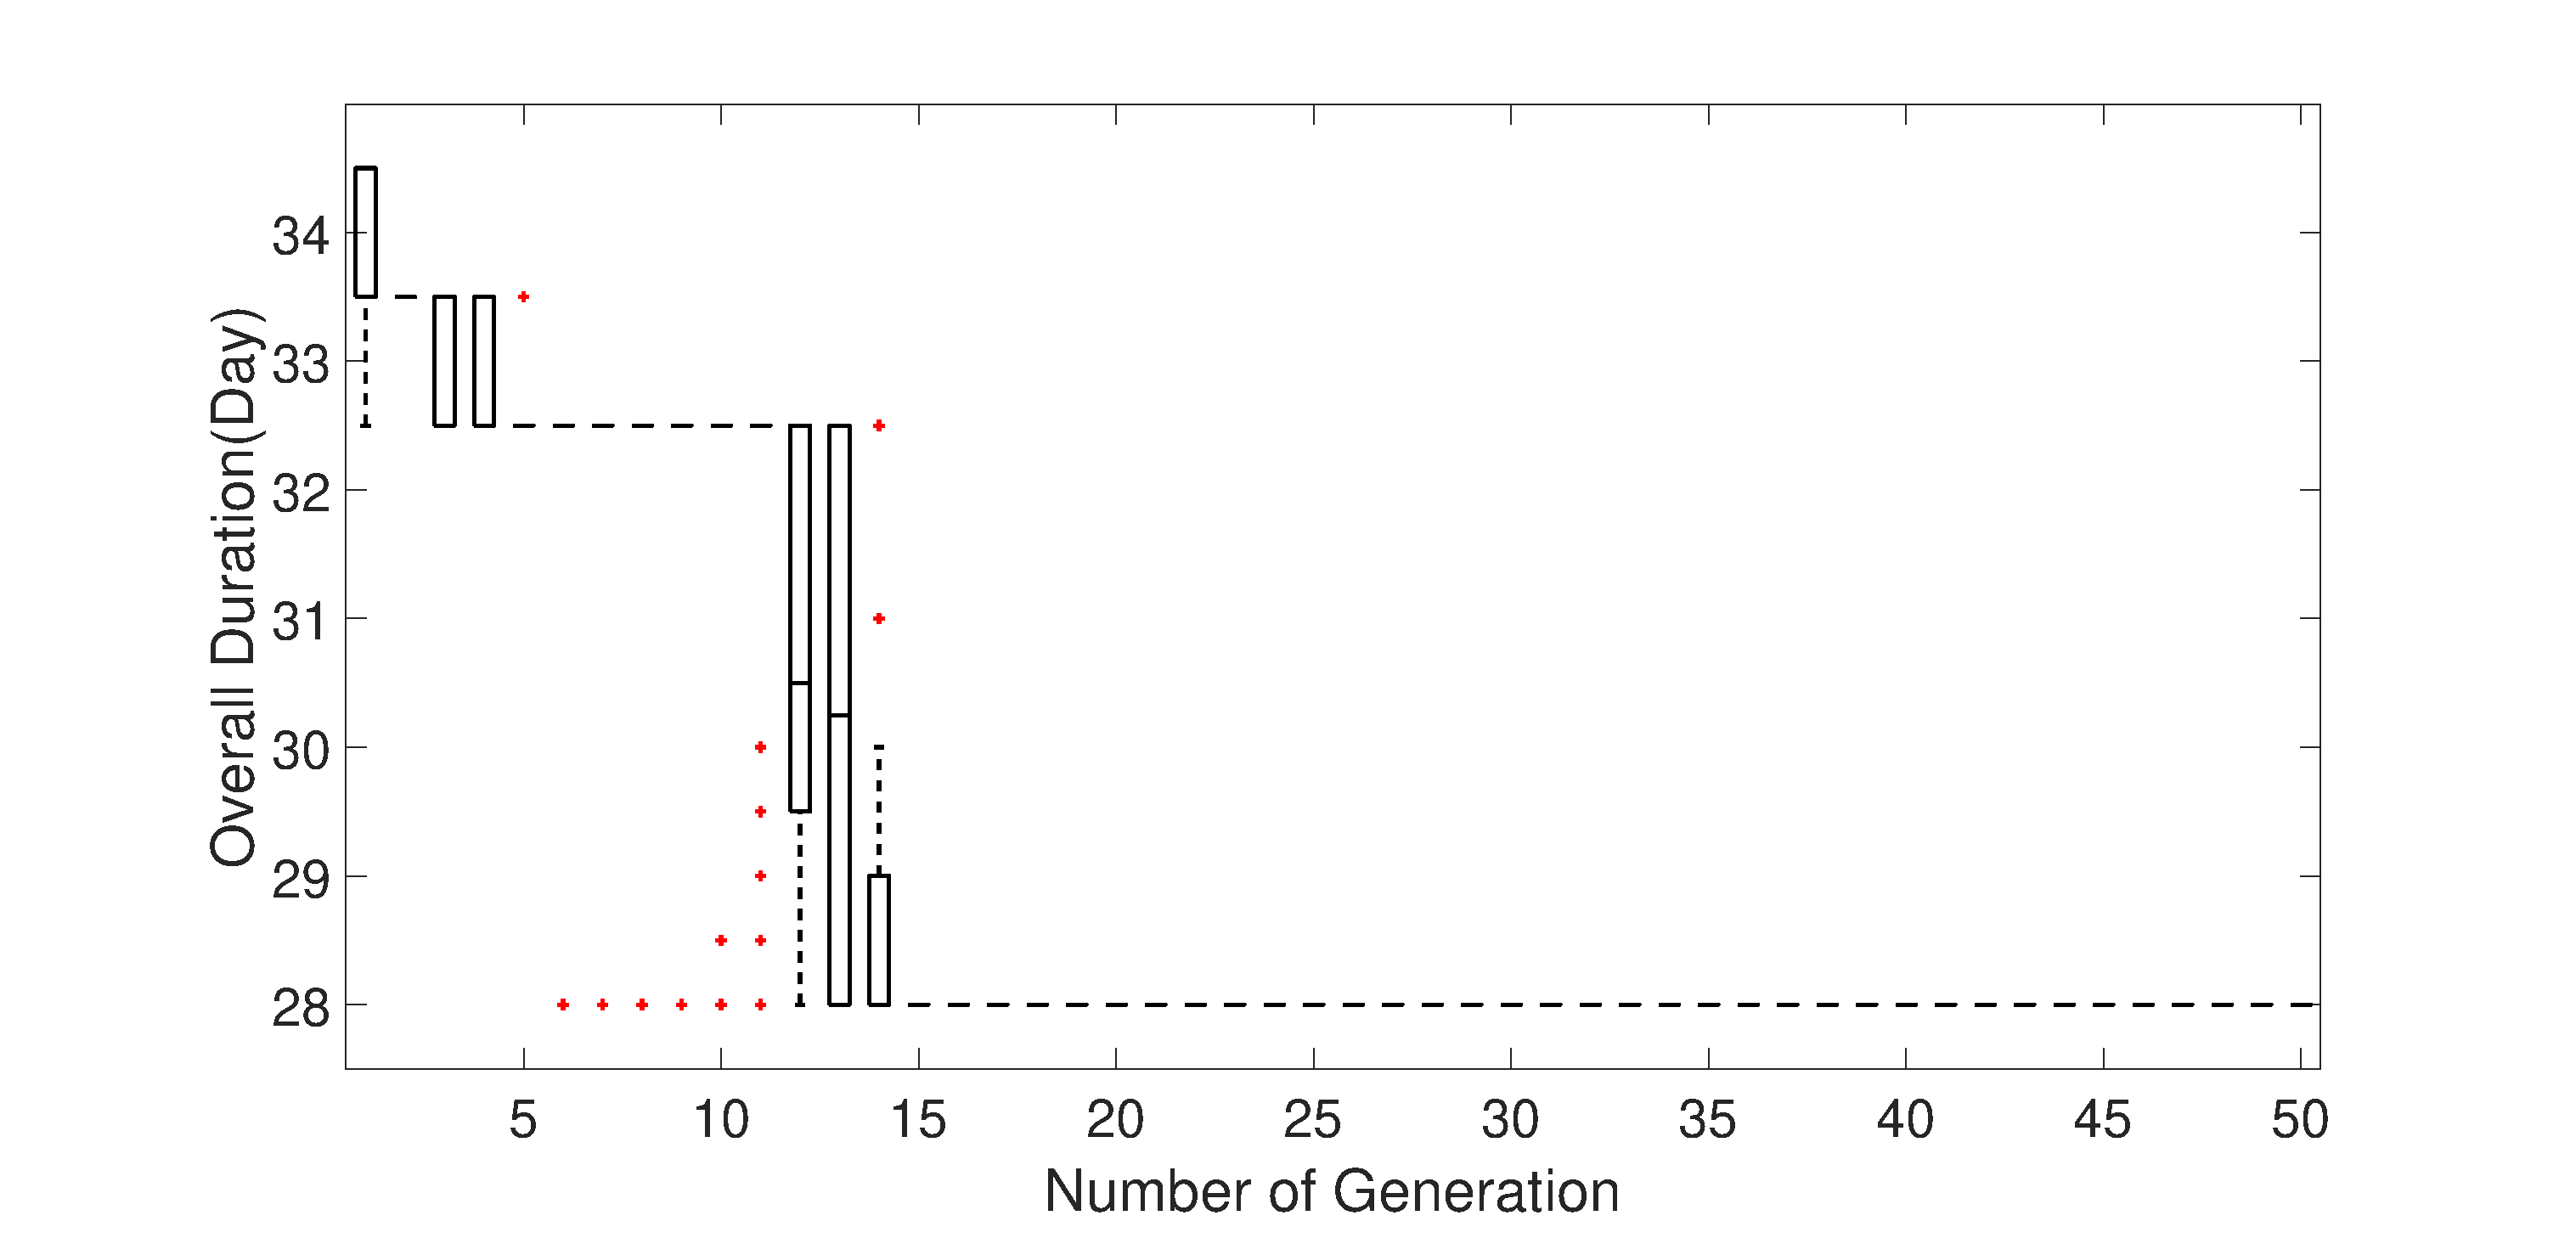
\includegraphics[width=0.8\textwidth]{figures/fig_pa3.eps}
  }
  \caption{caption}
  \label{fig:pj}
\end{figure}



Through the above analysis results of experimental data, we can accurately
answer \textbf{RQ1}. In the project management problems, the evolutionary
algorithm does have a good optimization and improvement.


\subsection{Efficiency Experiment for Algorithm}
%
In order to answer \textbf{RQ2}, this section conduct a efficiency experiment
that compares the efficiency between the parallel evolutionary algorithm and the
sequential one.

The hardware environment of this experiment is as follows: the runtime
environment that execute the sequential evolutionary algorithm is the Intel i7
series CPU (abbreviated as CPU). The runtime environment of the parallel
evolutionary algorithm is the NVidia GeForce series GPU (abbreviated as GPU
). CPU and GPU detailed configuration comparison see Table \ref{tab:cpugpu}. The
software environment of this experiment is: Window 7 Ultimate Service Pack 1,
Microsoft Visual Studio 2012 C++ Compiler, CUDA 7.0.28 Runtime compilation
environment.

\begin{table}[!ht]
  \centering
  \caption{Hardware Configuration Comparison}
  \label{tab:cpugpu}
  \begin{tabular}{c|c}
    \hline
    CPU & GPU  \\
    \hline
    \hspace{.5cm} Intel i7 CPU 870 \hspace{.5cm} & \hspace{.5cm} GeForce GTX 970 \hspace{.5cm} \\
    2.93 GHz &:q 1.27 GHz \\
    8 cores & 1664 cores \\
    \hline
  \end{tabular}
\end{table}

The initial configuration of the two versions is the identical, which the number
of population is 1000 and the number of generation is 100. Each generation
includes crossover, mutation and selection. A timer is set to record the total
time consuming of the algorithms. The timer starts after loading initial data
and ends after the result is calculated. This allows us to count the total
computational time both in the sequential environment and the parallel
environment under the same criteria.

<<<<<<< Updated upstream
\begin{figure}[!ht]
=======
\begin{table}
  \centering
  \caption{Three Project's Time of Calculation}
  \label{tab:consuming}
  \begin{tabular}{ccc|cc|cc}
    \hline
    & \multicolumn{2}{c}{ \emph{A-Input} } & \multicolumn{2}{c}{ \emph{B-DBUpgrade} } & \multicolumn{2}{c}{ \emph{C-SmartPrice} } \\
    \hline
      Time(ms) & \hspace{.25cm} CPU \hspace{.25cm} & \hspace{.25cm} GPU \hspace{.25cm} & \hspace{.25cm} CPU \hspace{.25cm} & \hspace{.25cm} GPU \hspace{.25cm} & \hspace{.25cm} CPU \hspace{.25cm} & \hspace{.25cm} GPU \hspace{.25cm}\\
    \hline
     1 & 7991.8 & 8431.8 & 45225.1 & 21217.5 & 29642.9 & 14844.3 \\
     2 & 8431.8 & 4279.7 & 44832.1 & 21377.9 & 28733.7 & 14543.6 \\
     3 & 7504.1 & 3947.9 & 44934.9 & 21227.2 & 28657.9 & 15003.4 \\
     4 & 7442.1 & 4642.5 & 44197.1 & 21340.3 & 29489.5 & 14882.8 \\
     5 & 7376.9 & 4263.8 & 45233.7 & 22448.2 & 29379.5 & 14921.5 \\
     6 & 7385.4 & 4188.6 & 45197.5 & 20956.1 & 28687.9 & 14723.3 \\
     7 & 8238.8 & 4540.2 & 45305.4 & 21777.2 & 29786.3 & 13978.8 \\
     8 & 7470.7 & 4226.4 & 45322.8 & 21147.1 & 31231.7 & 14811.1 \\
     9 & 7604.8 & 3778.2 & 45040.7 & 21004.7 & 28319.7 & 14292.0 \\
     10  & 7451.9 & 4712.4 & 45970.6 & 21500.9 & 28322.1 & 14429.7 \\
     Avg. & 7689.8 & 4268.2 & 45126.0 & 21399.7 & 29225.1 & 14643.1 \\
    \hline
  \end{tabular}
\end{table}


\begin{figure}[!htb]
  \centering
  \subfigure[\emph{A-Input}'s Time of Calculation]{
    \label{fig:co:a}
    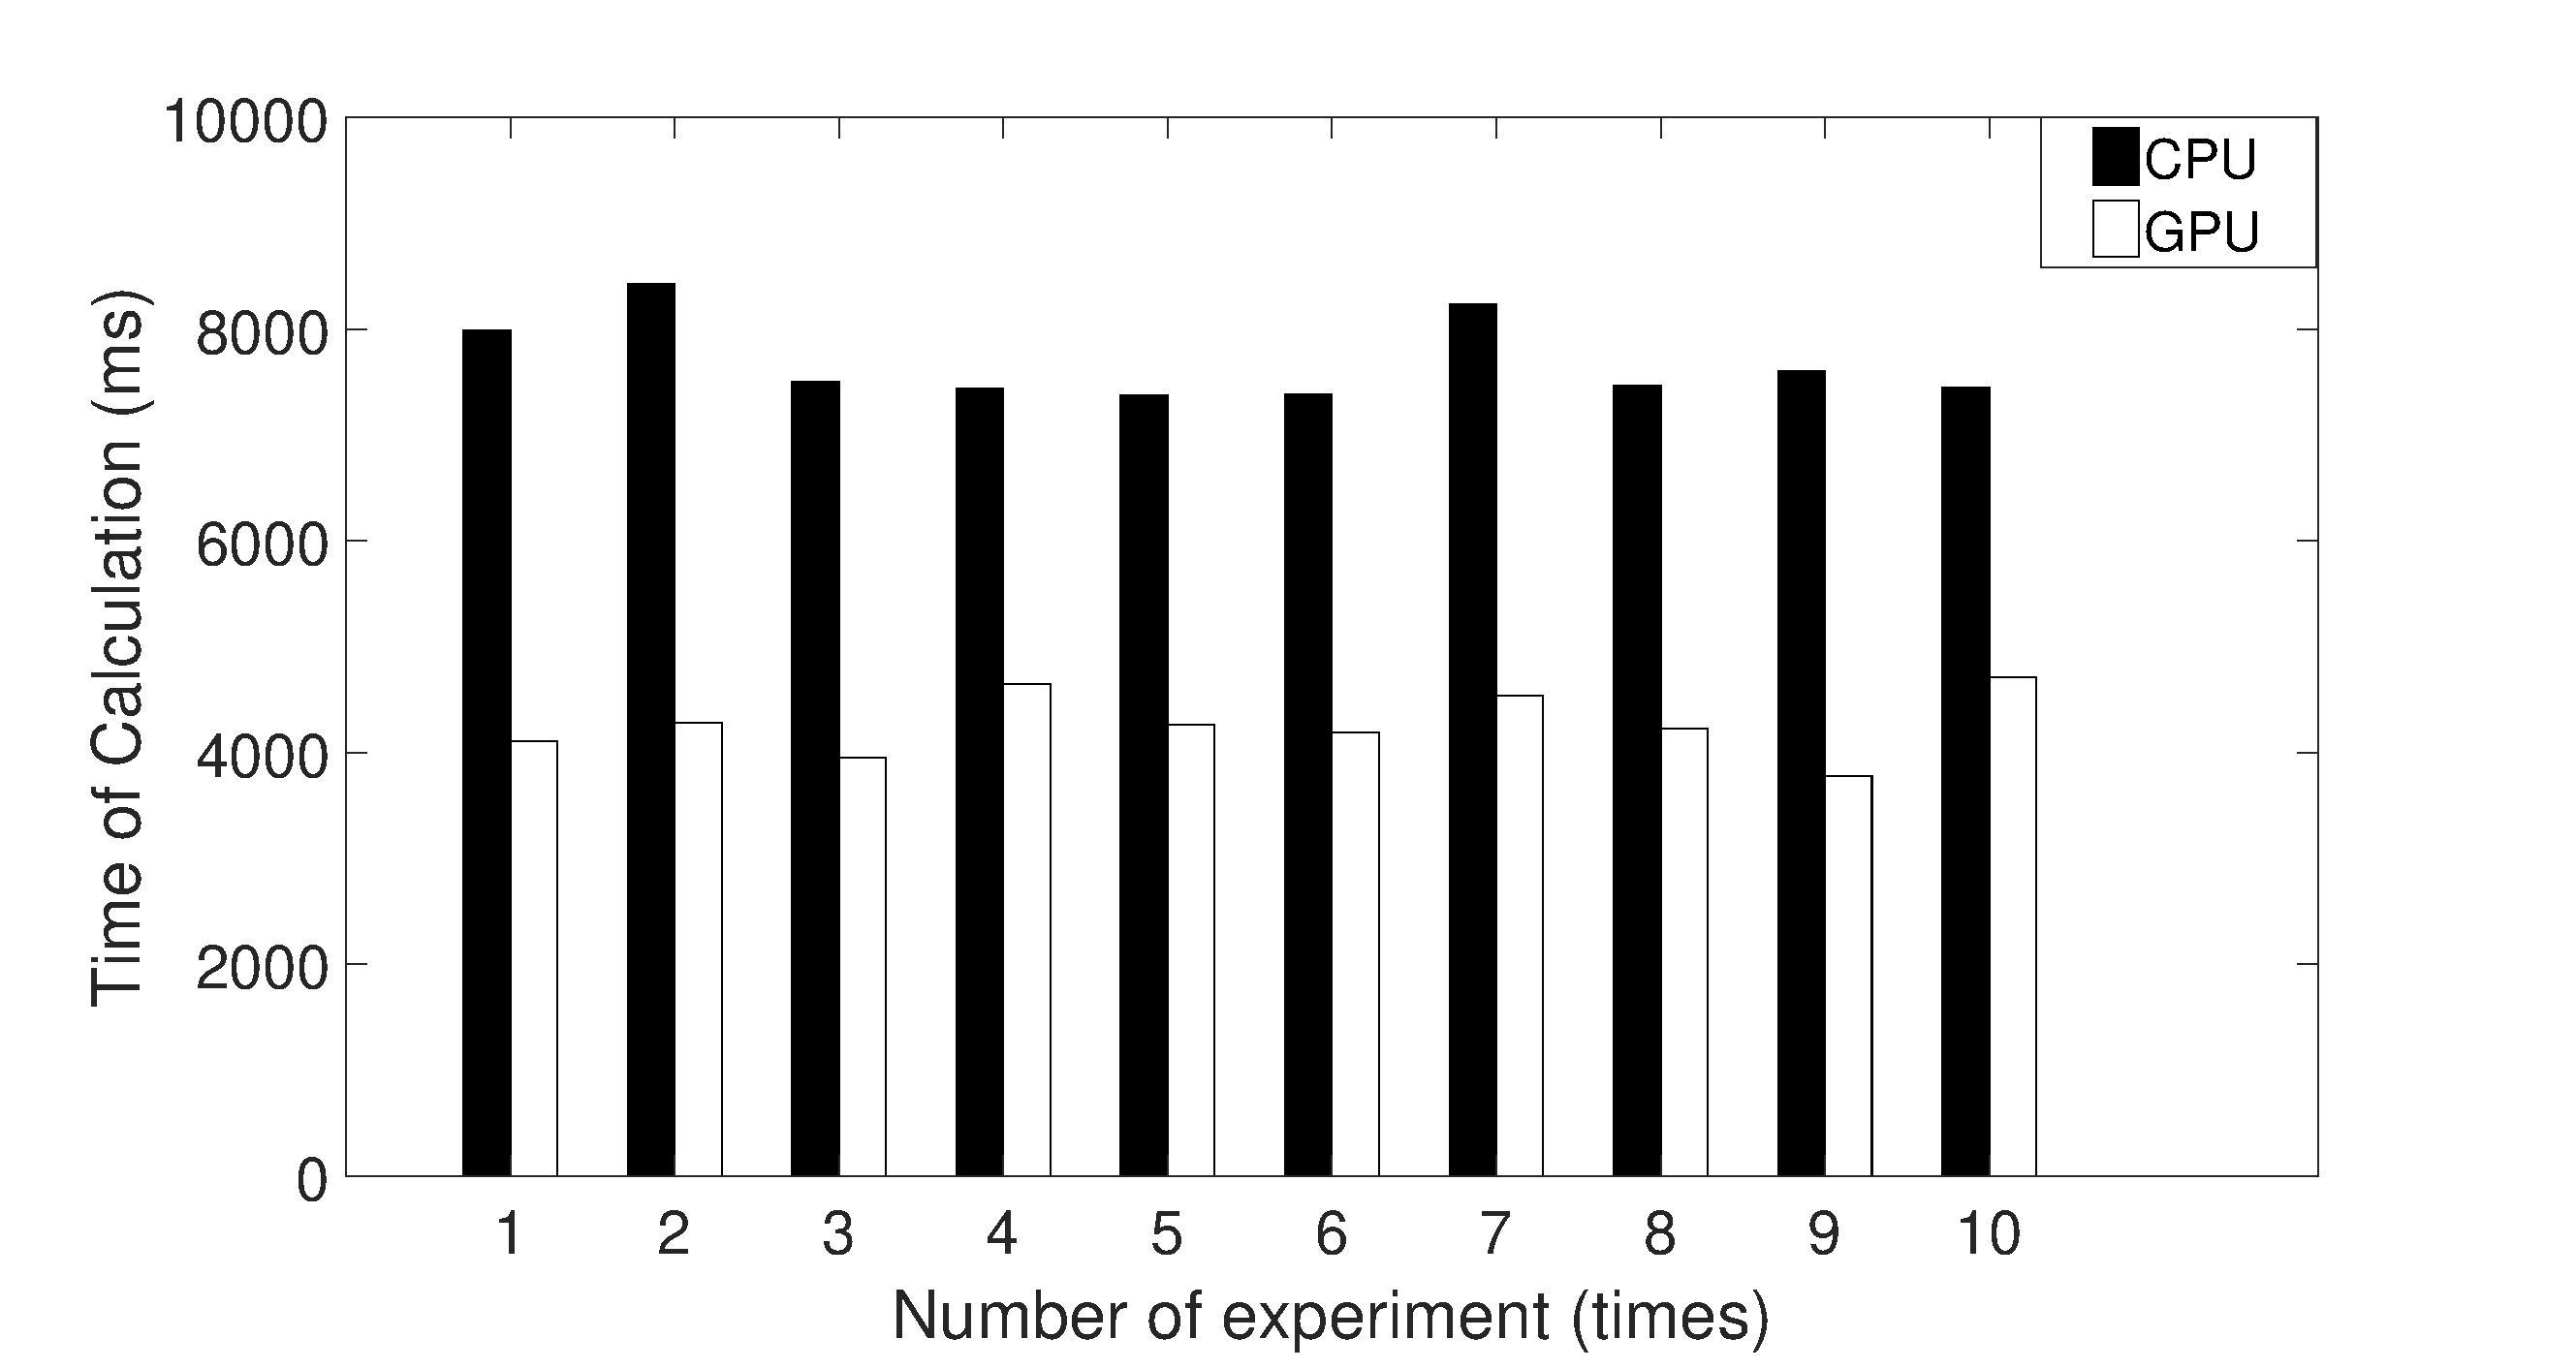
\includegraphics[width=0.8\textwidth]{figures/fig_co1.eps}
  }
  \subfigure[\emph{B-DBUpgrade}'s Time of Calculation]{
    \label{fig:co:b}
    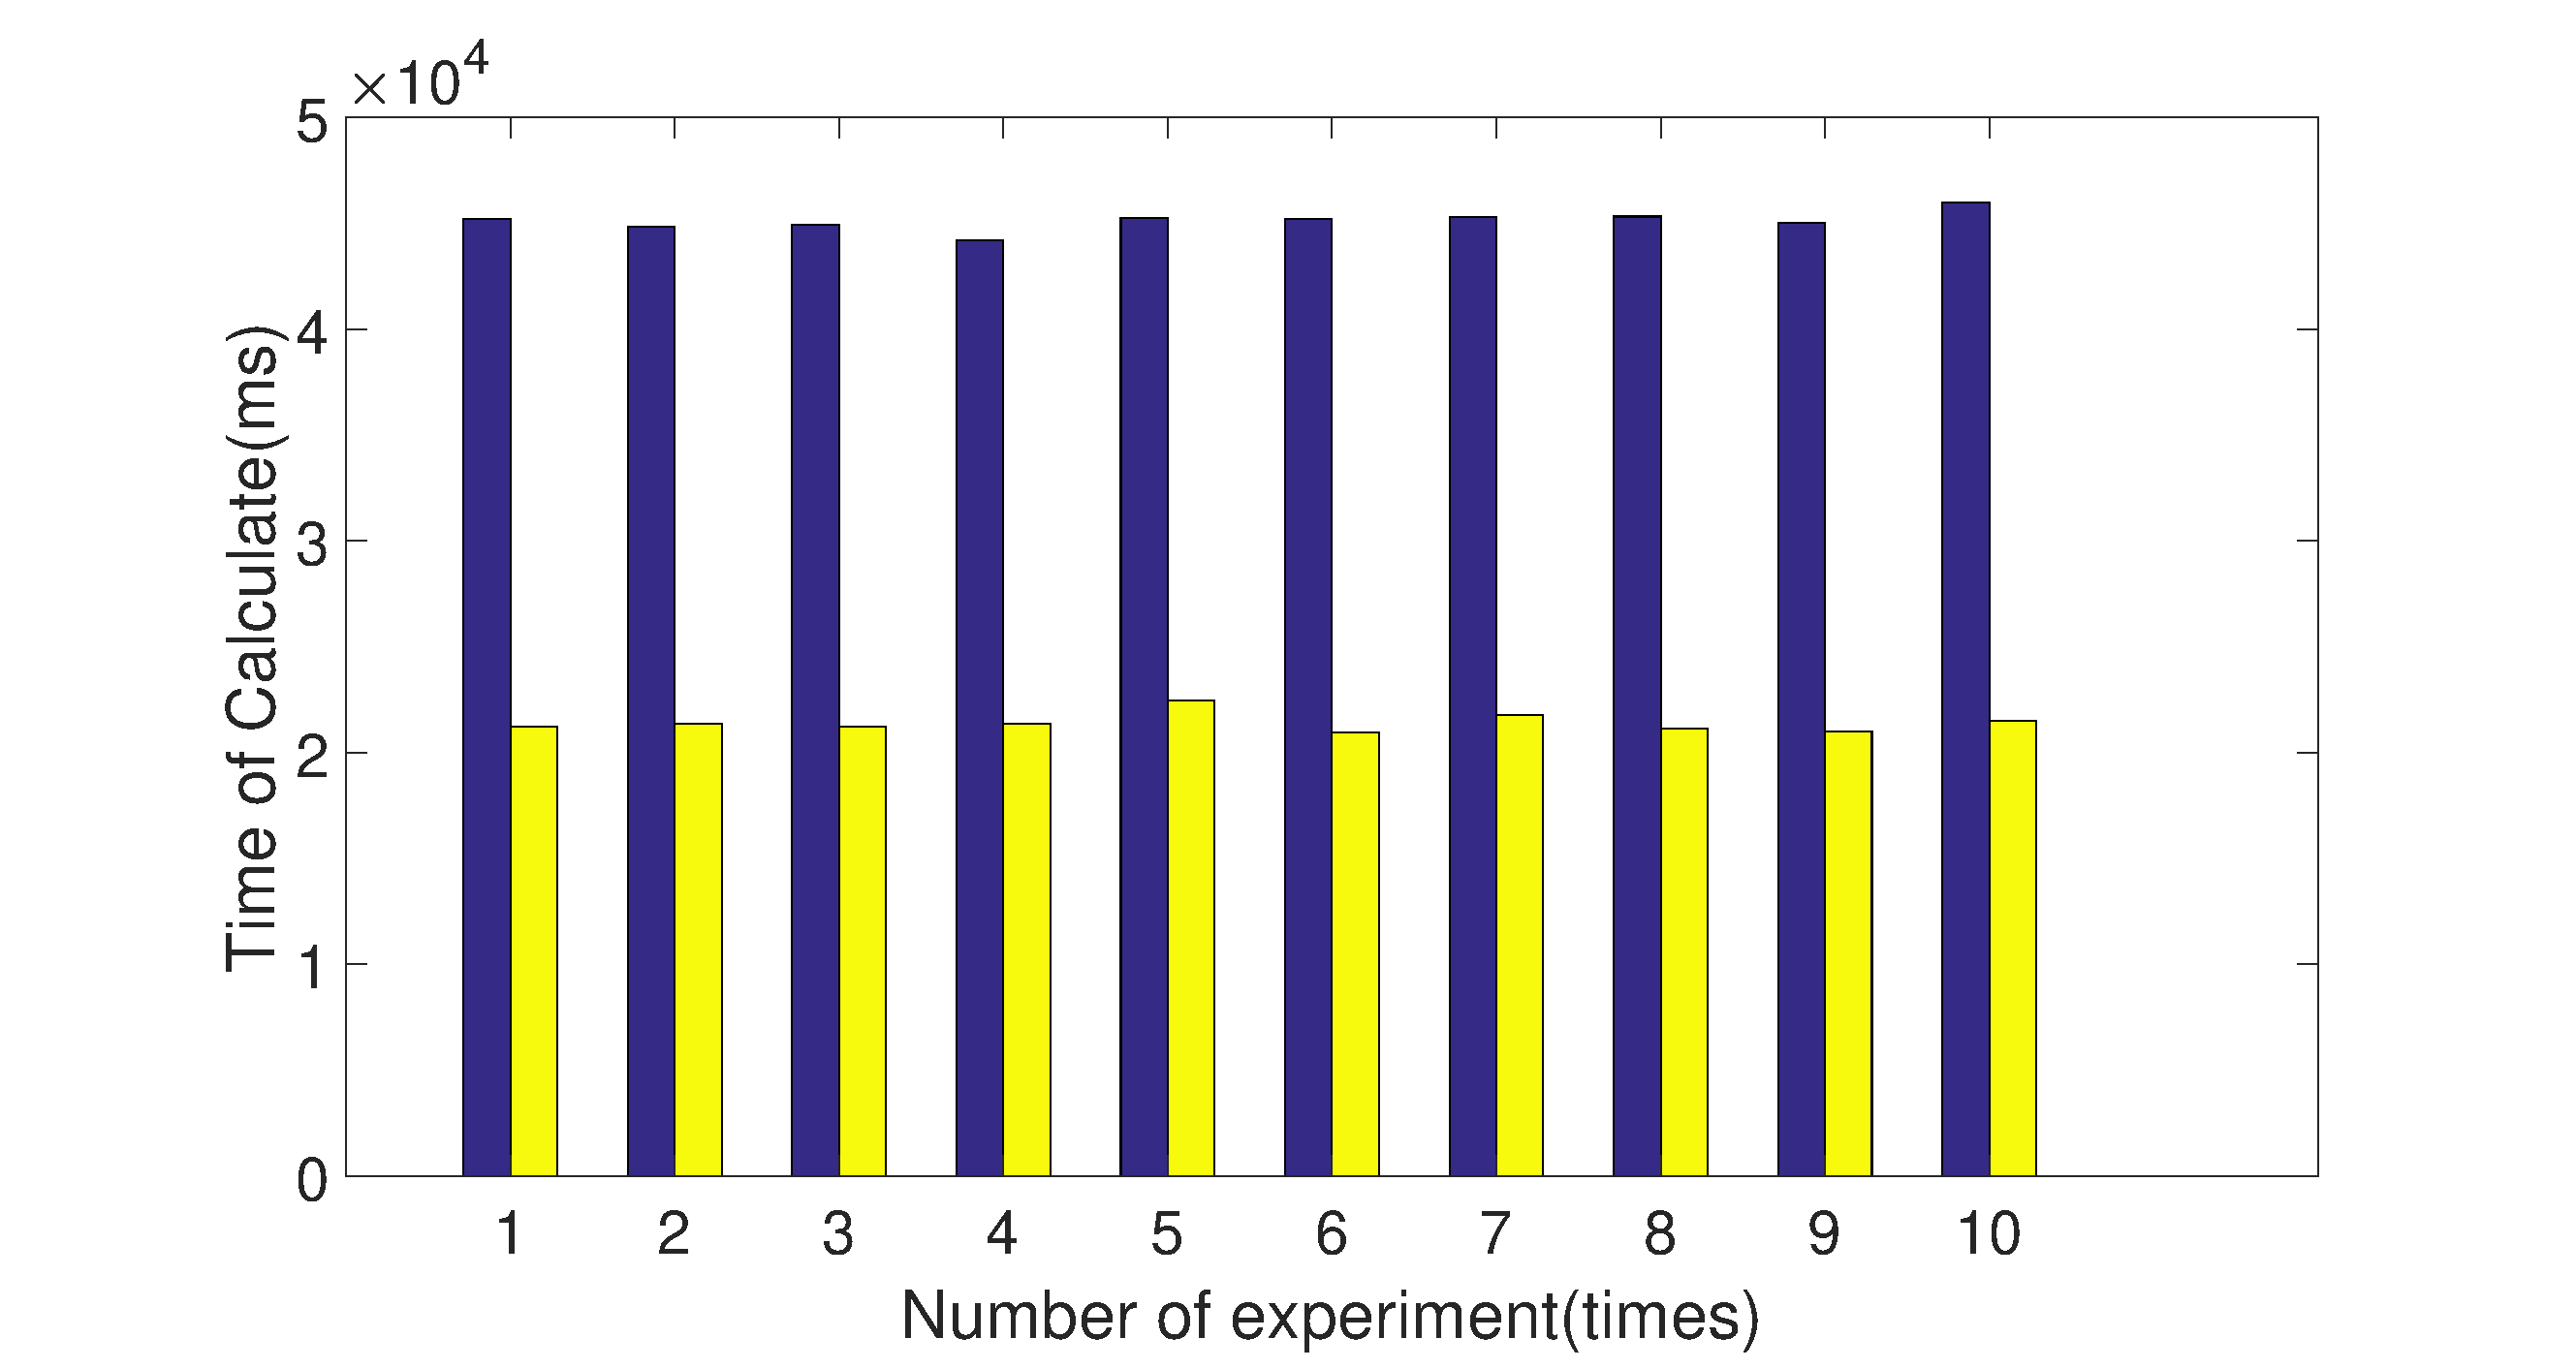
\includegraphics[width=0.8\textwidth]{figures/fig_co2.eps}
  }
  \subfigure[\emph{C-SmartPrice}'s Time of Calculation]{
    \label{fig:co:c}
    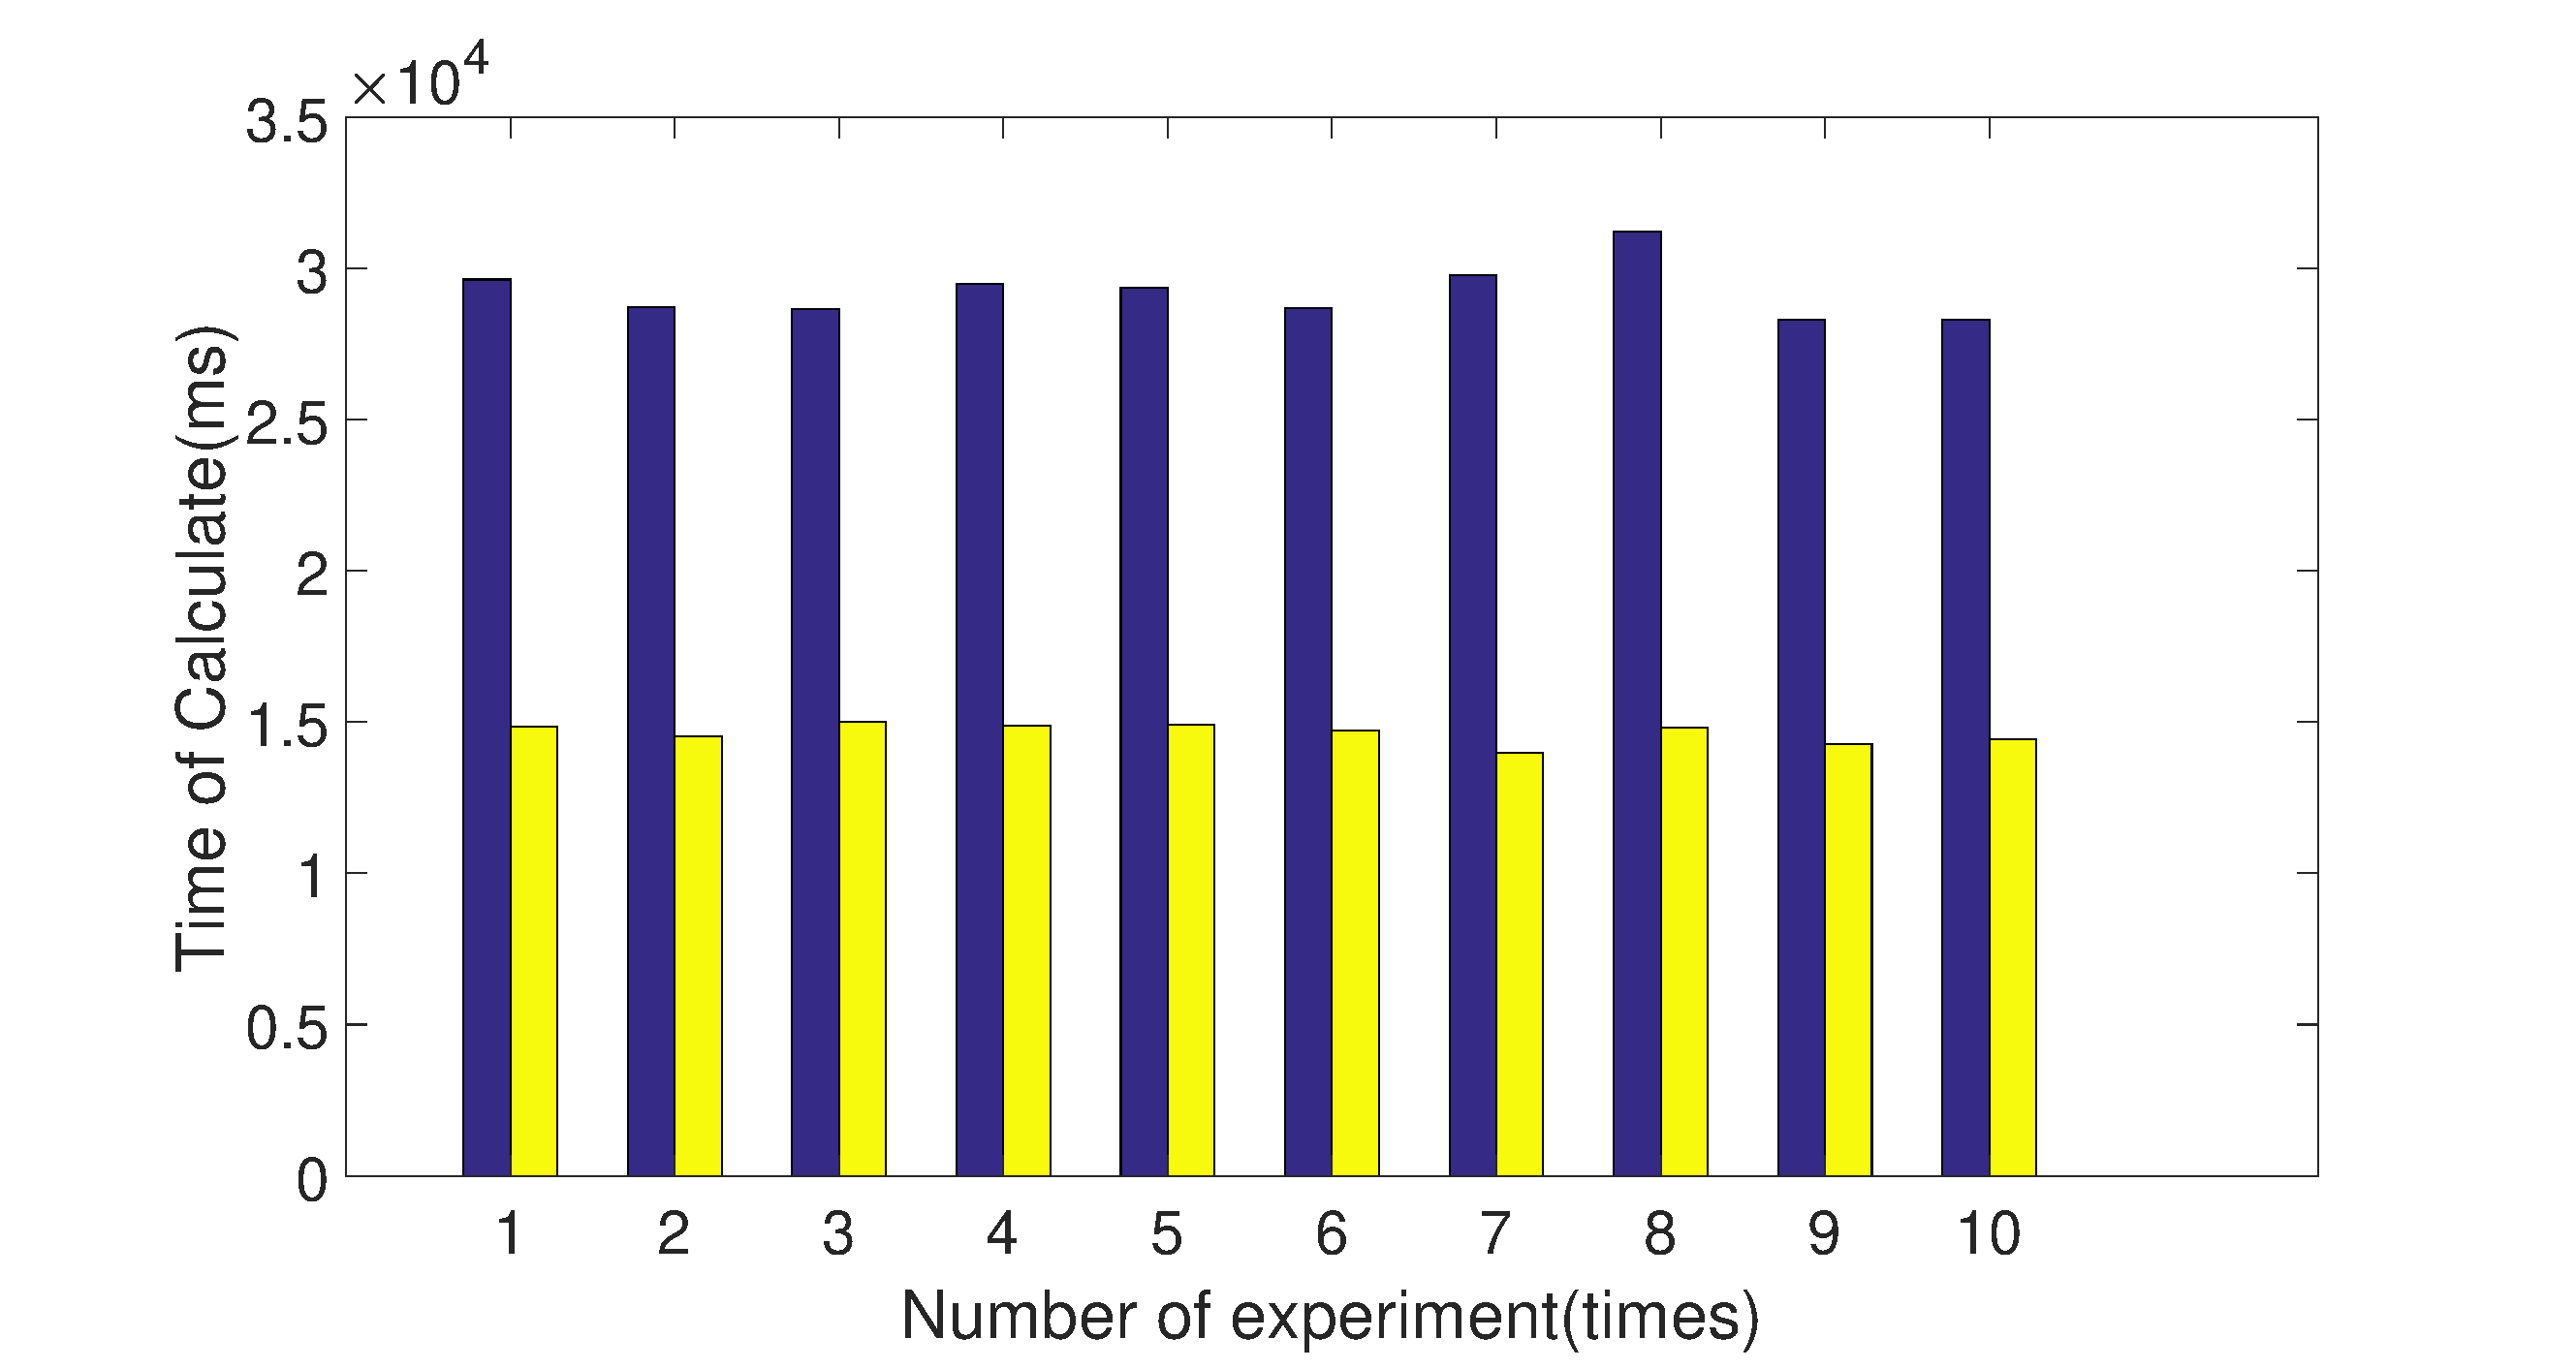
\includegraphics[width=0.8\textwidth]{figures/fig_co3.eps}
  }
  \caption{Time Comparison of \emph{CPU} and \emph{GPU}}
  \label{fig:co}
\end{figure}



The efficiency experiments are repeated $10$ times.  The final result of
\emph{A-Input}, \emph{B-DBUpgrade} and \emph{C-SmartPrice} are shown in figures
\ref{fig:co}. It can be seen from the figures that the time-consuming of the
sequential algorithm on CPU is roughly twice as long as the parallel algorithm
on GPU. So it can be a good answer to \textbf{RQ2} that parallel evolutionary
algorithm can improve the efficiency on computing the project management
problems.

